\documentclass[../../main.tex]{subfiles}
\begin{document}

\subsection*{10.16}
Un filo indefinito è percorso dalla corrente $i(t) = i_0\ e^{-\frac{t}{\tau}}$ con $i_0 = 10\ A$ e $\tau = 5\ s$ e si trova in un piano in cui c'è una spira rettangolare di lati $a = 6\ cm$, $b = 12\ cm$, con il lato più vicino parallelo al filo alla distanza $r = 4\ cm$.\\
Calcolare la f.e.m. indotta nella spira e la carica q che percorre la spira nell'intervallo di tempo da zero a $+\infty$, se essa ha una resistenza $R = 2\ \Omega$.\\
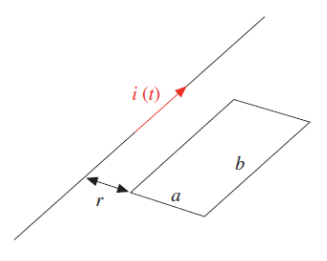
\includegraphics[scale=0.3]{e_10_16.png}
\subsubsection*{Formule utilizzate}
$B(t) = \frac{\mu_0 i(t)}{2\pi r}$\\
\subsubsection*{Soluzione punto a}
Il filo produce un campo magnetico B.\\
$B(t) = \frac{\mu_0 i(t)}{2\pi (x + r)}$\\
$\Phi(B(t)) = \int_0^a \frac{\mu_0i(t)}{2\pi (x+r)}b dx$\\
Il campo magnetico è ortogonale alla spira quindi l'angolo fra $u_n$ e B è tale da dare un coseno = 1.\\
$\Phi(t) = \frac{\mu_o ib}{2\pi}ln\left(1+\frac{a}{r}\right)$
Dalla legge di Lenz:\\
$\varepsilon_i = -\frac{d\Phi(t)}{dt} = \frac{\mu_0 ib}{2\pi r} e^{-\frac{t}{\tau}}ln\left(1+\frac{a}{r}\right) = 4.4 * 10^{-8}\ e^{-\frac{t}{5}}\ V$
\subsubsection*{Soluzione punto b}
Nella spira troveremo:\\
$i_{spira} = \frac{\varepsilon_i}{R} = 2.2 * 10^{-8}\ e^{-\frac{t}{5}}\ A$\\
E la carica che fluisce è:\\
$q = \int_0^\infty i_{spira}(t)dt = 1.1*10^{-7}C$\\
Per la legge di felici:\\
$q = \frac{\Delta\Phi}{R} = 1.1 * 10^{-7}\ C$
\newpage

\end{document}